\documentclass[11pt]{article}
\usepackage[margin=1in]{geometry}
\usepackage{amsmath,amssymb}
\usepackage{graphicx}
\usepackage{float}
\usepackage[hidelinks]{hyperref}
\graphicspath{{site_sweep/figures/}}
\title{Hard AbsTopK gate on MNIST: after a linear layer against on the input}
\author{}
\date{2026-10-26}

\begin{document}
\maketitle

\begin{figure}[H]
\centering
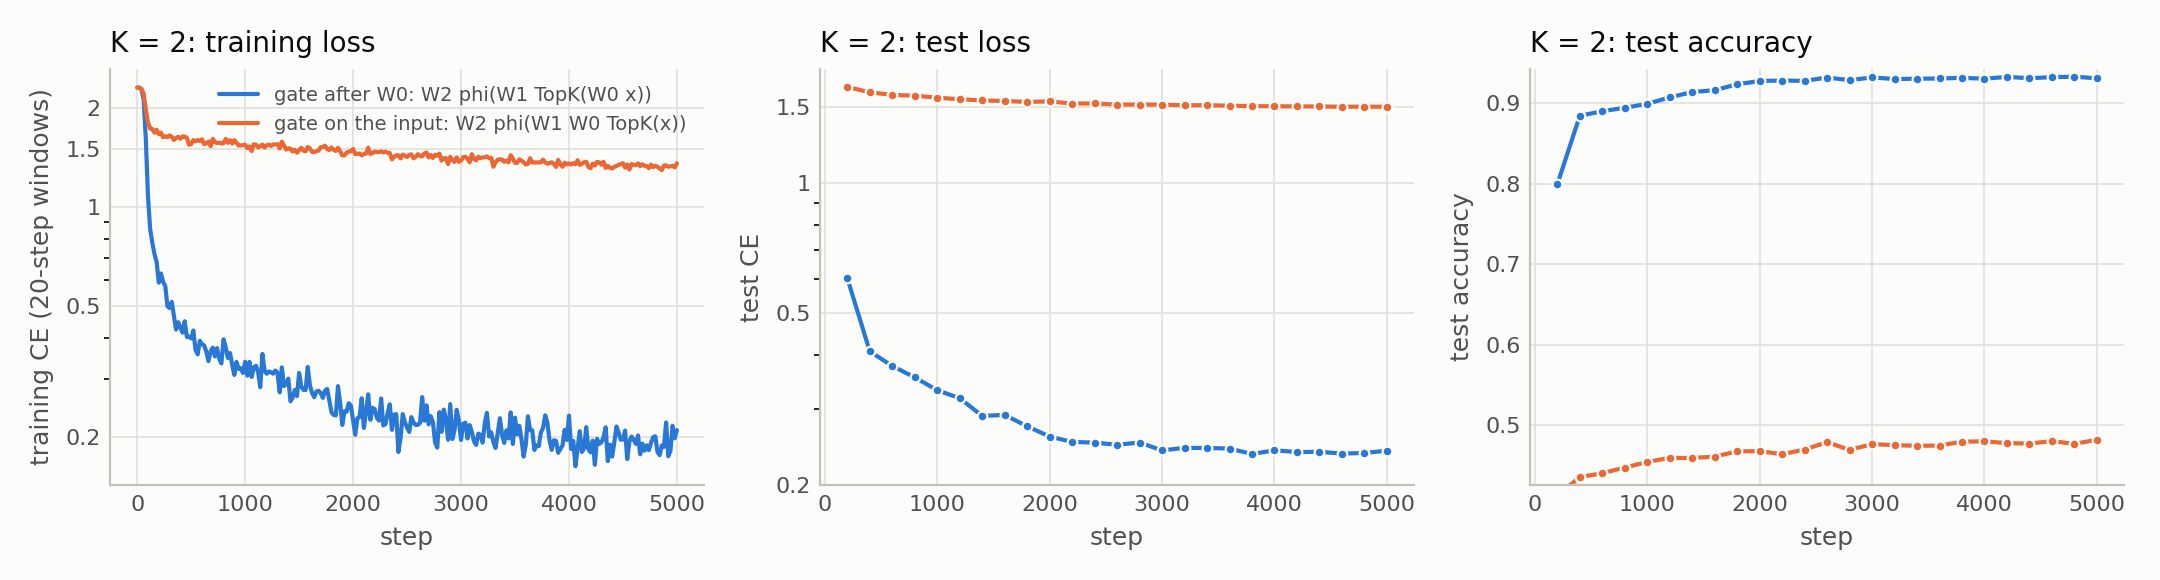
\includegraphics[width=\linewidth]{curves_k2.png}
\caption{$K = 2$: training CE (left, log scale, 20-step window means), test CE (middle, log scale, every 200 steps) and test accuracy (right) for $z = W_2\,\phi(W_1\,\mathrm{AbsTopK}_K(W_0 x))$ (gate after $W_0$) and $z = W_2\,\phi(W_1 W_0\,\mathrm{AbsTopK}_K(x))$ (gate on the input); $W_0$ is $784 \times 784$ without bias, hidden width 1024, hard backward, 5000 steps.}
\label{fig:k2}
\end{figure}

\begin{figure}[H]
\centering
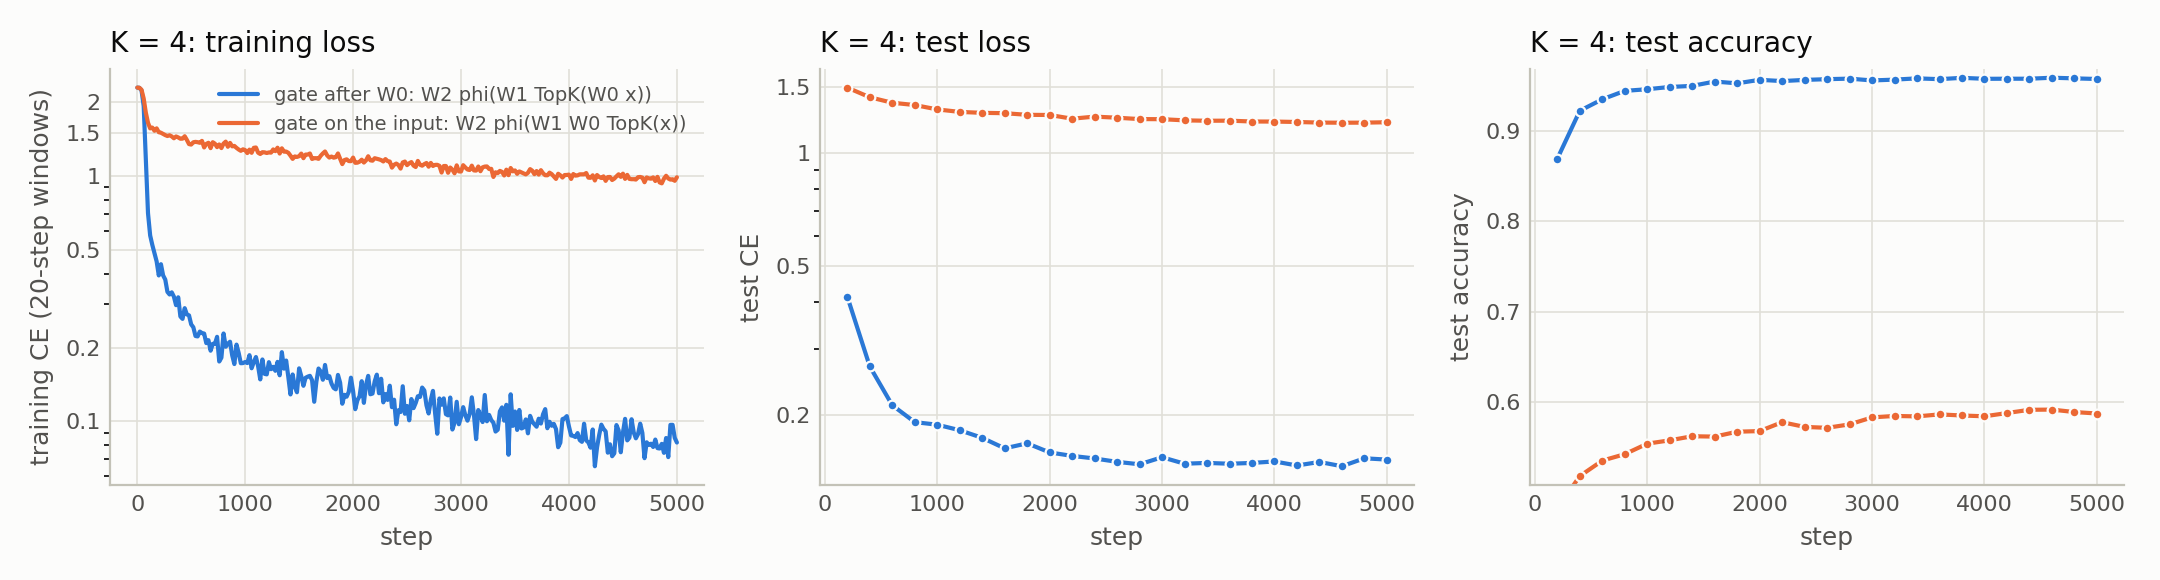
\includegraphics[width=\linewidth]{curves_k4.png}
\caption{$K = 4$: as Figure~\ref{fig:k2}.}
\label{fig:k4}
\end{figure}

\begin{figure}[H]
\centering
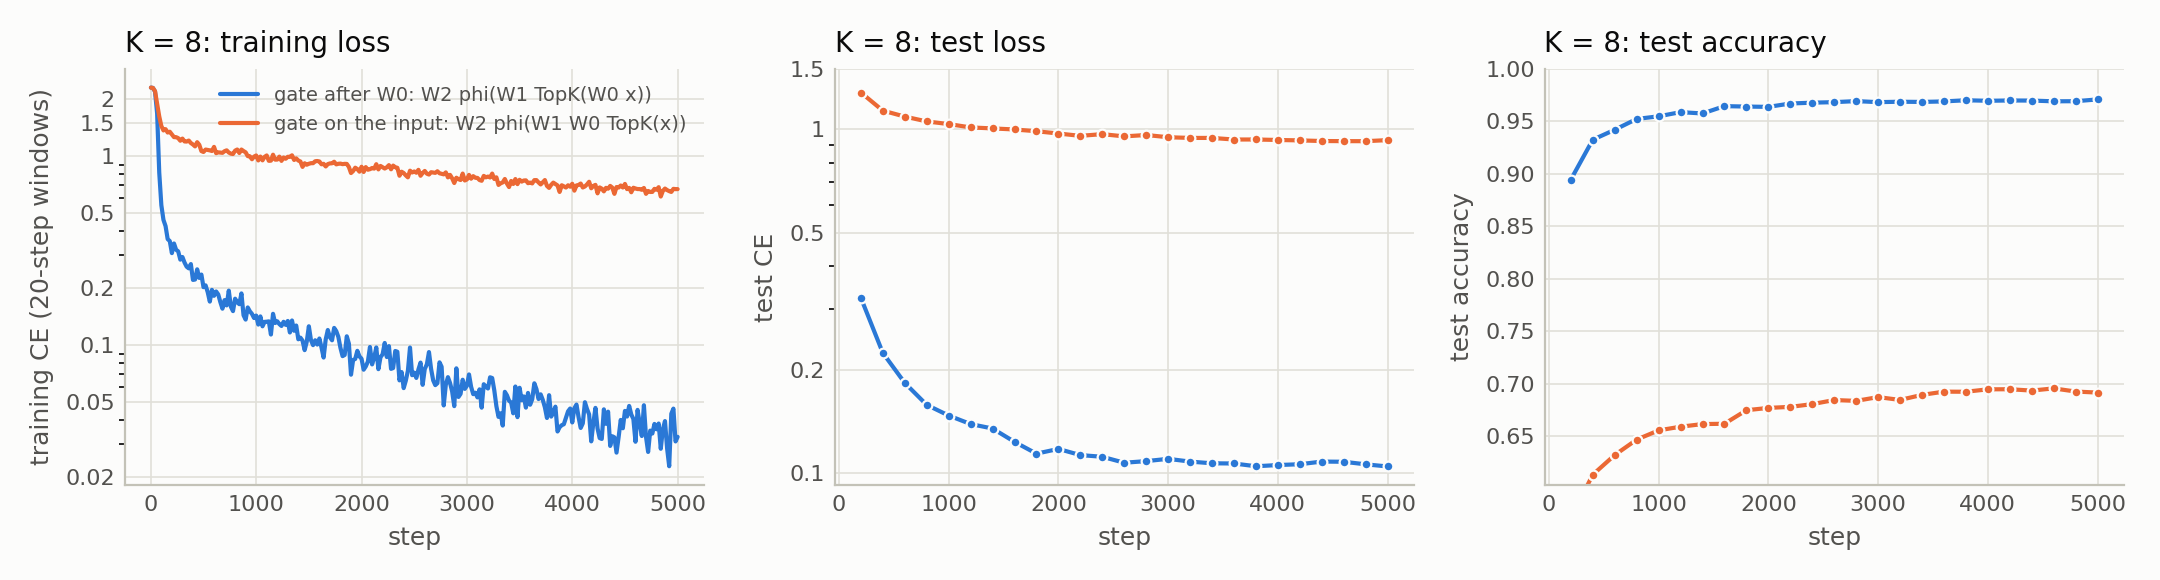
\includegraphics[width=\linewidth]{curves_k8.png}
\caption{$K = 8$: as Figure~\ref{fig:k2}.}
\label{fig:k8}
\end{figure}

\begin{figure}[H]
\centering
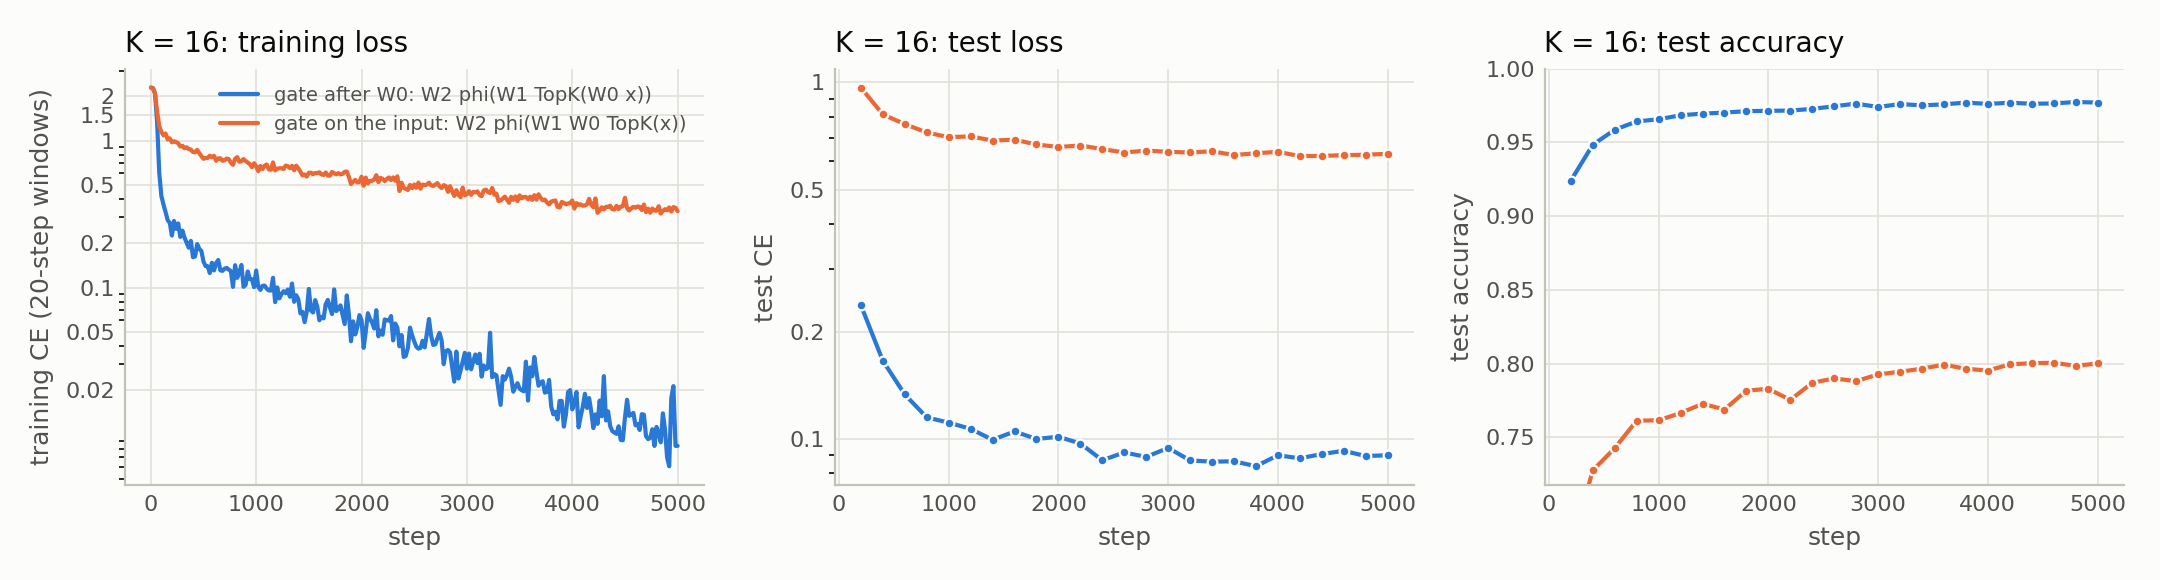
\includegraphics[width=\linewidth]{curves_k16.png}
\caption{$K = 16$: as Figure~\ref{fig:k2}.}
\label{fig:k16}
\end{figure}

\end{document}
